After getting the binary images of the vascular structures, we apply
the centerline extraction method using fast marching based on Hassouna
\cite{Hassouna}'s and Jakob \cite{Jakob}'s  work. They use fast
marching method to obtain an accurate solution of Eikonal equation
known as

$$|\nabla T| F = 1 , \; s.t.\; T(\Gamma_{0})=0$$

where  $\Gamma$ stands for the closed interface that separates one region
from another. Hassouna et al.~\cite{Hassouna} proposed an improved version
of the fast marching method with high accuracy called multistencils fast
marching(MSFM). By solving the Eikonal Equation at each point under several
stencils which cover 8 neighbours in 2D space and 26 in 3D space and picking
up the one which satisfies the upwind condition most, they can achieve
better accuracy. For stencils not aligned with the natural coordinate
system, Eikonal equation is derived using directional derivatives and solved
using higher finite difference schemes.

Our approach is based on Jakob \cite{Jakob}'s  work. The 2D binary
image points can be divided into \textit{frozen} pixels which we
compute distances at their neighbours and \textit{narrow band} pixels.
For each iteration, the \textit{narrow band} pixels having the
smallest distance value is frozen and distances are computed from its
neighbours. Progressively, the \textit{narrow band} pixels propagate
from the initial condition and the freezing pixels follow them along,
finally, when all points are frozen, the method vanishes. During the
procedure, we use the method proposed as Hassouna \cite{Hassouna} to
compute the distances and implement a custom unsorted binary tree
which performs like a normal binary sorted tree to select the minimum
distance in every MSFM iteration.

During the centerline tracking, every point in each line is tracked and the
bifurcations are recorded, finally we can get a vessel centerline tree
including all bifurcations as shown in Figure \ref{fig:centerline}. The left
image is the binary image representing the centerlines of the vessels, the
right is the original image with colored centerlines. Each red cross
represents one bifurcation and each color represents one single centerline.

\begin{figure}
  \centering
  % Requires \usepackage{graphicx}
  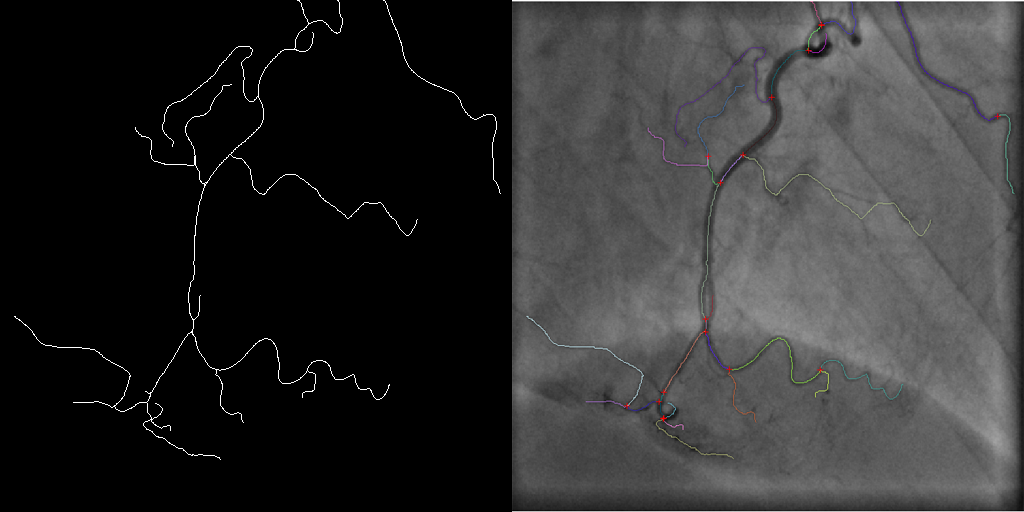
\includegraphics[width=3.0in]{centerline.png}\\
  \caption{Binary and Colored Centerlines}\label{fig:centerline}
\end{figure}
